% Diagram for the report (sequence). Build: see build.sh in this folder.
\documentclass[12pt]{standalone}
% Shared style of every diagram and chart in the report.
% Each agent keeps the same colour in every figure.
% The diagrams are drawn here, not in main.tex, so the report itself does not
% load TikZ: it includes the built PDFs and compiles within Overleaf's time limit.
\usepackage{amsmath,amssymb}
\usepackage{xcolor}
\usepackage{tikz}
\usetikzlibrary{positioning,arrows.meta,shapes.geometric,shapes.misc,fit,calc,backgrounds}
\usepackage{pgfplots}
\pgfplotsset{compat=1.18}

% Same text width as the report (A4, 30 mm + 20 mm margins), for the charts.
\setlength{\textwidth}{160mm}
\newcommand{\Rs}{Rs.\,}
\newcommand{\code}[1]{\texttt{\detokenize{#1}}}

\definecolor{ink}{HTML}{2B2B2B}
\definecolor{agAfill}{HTML}{E4F2E1}\definecolor{agAline}{HTML}{3E7D3A} % Agent 1 Document & Vendor
\definecolor{agBfill}{HTML}{FCEBD5}\definecolor{agBline}{HTML}{B8701D} % Agent 2 Approval & Inventory
\definecolor{agCfill}{HTML}{EEE4F4}\definecolor{agCline}{HTML}{6E4A8E} % Agent 3 Contract & Risk
\definecolor{agDfill}{HTML}{FBE4E4}\definecolor{agDline}{HTML}{A8474B} % Agent 4 Platform
\definecolor{infill}{HTML}{E8EDF6}\definecolor{inline}{HTML}{4F6188}    % infrastructure / data
\definecolor{exfill}{HTML}{F2F2F2}\definecolor{exline}{HTML}{6F6F6F}    % people and external systems
\definecolor{humfill}{HTML}{FFF6D6}\definecolor{humline}{HTML}{9A7B12}  % human decision points
\definecolor{chartA}{HTML}{9AA5B1}\definecolor{chartB}{HTML}{3F5E8C}    % chart: baseline / shipped

\tikzset{
  >={Stealth[length=2mm]},
  every picture/.style={font=\footnotesize, line width=0.6pt, draw=ink, text=ink},
  nohyph/.style={execute at begin node={\hyphenpenalty=10000\exhyphenpenalty=10000}},
  box/.style={nohyph, draw, rounded corners=2pt, align=center, inner sep=3pt, minimum height=8mm},
  agA/.style={box, fill=agAfill, draw=agAline},
  agB/.style={box, fill=agBfill, draw=agBline},
  agC/.style={box, fill=agCfill, draw=agCline},
  agD/.style={box, fill=agDfill, draw=agDline},
  infra/.style={box, fill=infill, draw=inline},
  ext/.style={box, fill=exfill, draw=exline},
  human/.style={box, fill=humfill, draw=humline},
  decision/.style={nohyph, diamond, aspect=2.2, draw=humline, fill=humfill, align=center, inner sep=1pt},
  flow/.style={->, draw=ink},
  dflow/.style={->, draw=ink, dashed},
  lbl/.style={font=\scriptsize\itshape, fill=white, inner sep=1pt},
  note/.style={font=\scriptsize\itshape, align=center},
}
\pgfplotsset{
  reportbars/.style={
    ybar, width=0.95\textwidth, height=6cm, ymin=0,
    enlarge x limits=0.18, bar width=11pt,
    ymajorgrids, grid style={draw=black!12},
    axis line style={draw=black!60}, tick style={draw=black!60},
    legend style={draw=none, font=\footnotesize, legend columns=-1, at={(0.5,1.03)}, anchor=south},
    tick label style={font=\footnotesize}, label style={font=\footnotesize},
    nodes near coords, every node near coord/.append style={font=\scriptsize},
    /tikz/every even column/.append style={column sep=0.6cm},
    legend image code/.code={\draw[#1, draw=none] (0cm,-0.1cm) rectangle (0.3cm,0.1cm);},
  },
}

\begin{document}
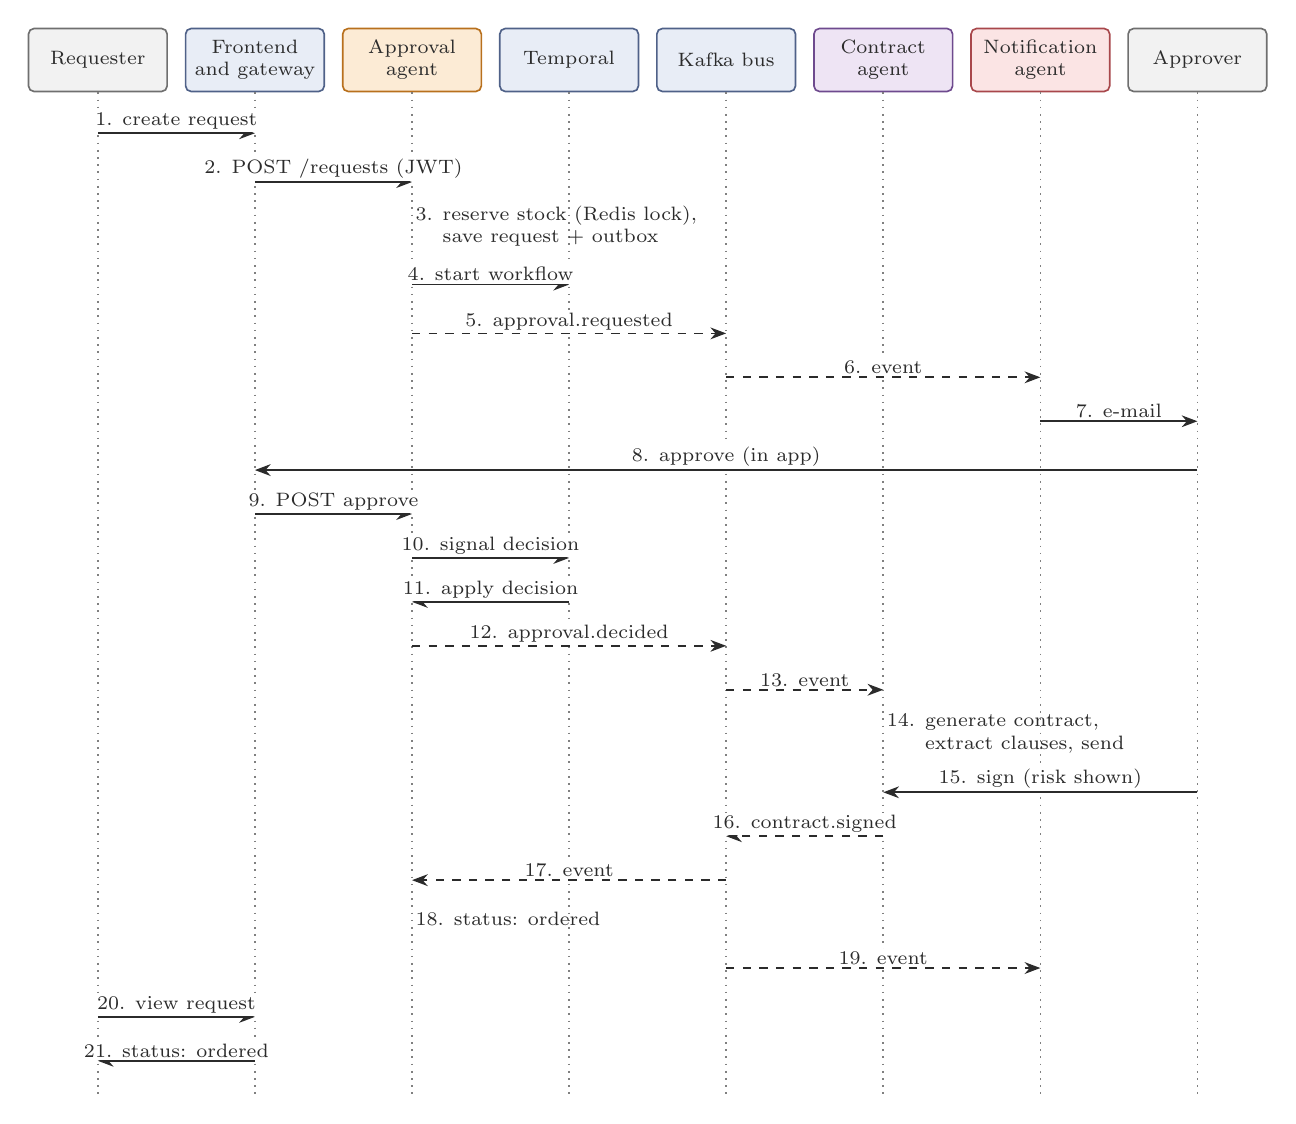
\begin{tikzpicture}[x=0.95cm, y=-0.62cm]
\tikzset{ll/.style={box, text width=1.55cm, minimum height=10mm, font=\scriptsize}, msg/.style={->, draw=ink}, amsg/.style={->, draw=ink, dashed}, ml/.style={font=\scriptsize, above, inner sep=1pt, fill=white}, self/.style={font=\scriptsize, right, inner sep=1pt, align=left}}
\foreach \x/\n/\t/\s in {0/rq/Requester/ext, 2.1/gw/Frontend and gateway/infra, 4.2/ap/Approval agent/agB, 6.3/tp/Temporal/infra, 8.4/kf/Kafka bus/infra, 10.5/ct/Contract agent/agC, 12.6/nt/Notification agent/agD, 14.7/av/Approver/ext}
  { \node[ll, \s] (\n) at (\x,0) {\t}; \draw[dotted, draw=black!50] (\n.south) -- (\x,21.2); }
\draw[msg] (0,1.5) -- node[ml] {1. create request} (2.1,1.5);
\draw[msg] (2.1,2.5) -- node[ml] {2. POST /requests (JWT)} (4.2,2.5);
\node[self] at (4.2,3.4) {3. reserve stock (Redis lock),\\\phantom{3. }save request + outbox};
\draw[msg] (4.2,4.6) -- node[ml] {4. start workflow} (6.3,4.6);
\draw[amsg] (4.2,5.6) -- node[ml] {5. approval.requested} (8.4,5.6);
\draw[amsg] (8.4,6.5) -- node[ml] {6. event} (12.6,6.5);
\draw[msg] (12.6,7.4) -- node[ml] {7. e-mail} (14.7,7.4);
\draw[msg] (14.7,8.4) -- node[ml] {8. approve (in app)} (2.1,8.4);
\draw[msg] (2.1,9.3) -- node[ml] {9. POST approve} (4.2,9.3);
\draw[msg] (4.2,10.2) -- node[ml] {10. signal decision} (6.3,10.2);
\draw[msg] (6.3,11.1) -- node[ml] {11. apply decision} (4.2,11.1);
\draw[amsg] (4.2,12.0) -- node[ml] {12. approval.decided} (8.4,12.0);
\draw[amsg] (8.4,12.9) -- node[ml] {13. event} (10.5,12.9);
\node[self] at (10.5,13.8) {14. generate contract,\\\phantom{14. }extract clauses, send};
\draw[msg] (14.7,15.0) -- node[ml] {15. sign (risk shown)} (10.5,15.0);
\draw[amsg] (10.5,15.9) -- node[ml] {16. contract.signed} (8.4,15.9);
\draw[amsg] (8.4,16.8) -- node[ml] {17. event} (4.2,16.8);
\node[self] at (4.2,17.6) {18. status: ordered};
\draw[amsg] (8.4,18.6) -- node[ml] {19. event} (12.6,18.6);
\draw[msg] (0,19.6) -- node[ml] {20. view request} (2.1,19.6);
\draw[msg] (2.1,20.5) -- node[ml] {21. status: ordered} (0,20.5);
\end{tikzpicture}
\end{document}
